\documentclass[11pt]{beamer}
\usetheme{Antibes}
\usepackage[utf8]{inputenc}
\usepackage[english]{babel}
\usepackage{amsmath}
\usepackage{amsfonts}
\usepackage{amssymb}
\usepackage{graphicx}
\author{Boris Arnoux}
\title{Composable ML}
%\setbeamercovered{transparent} 
%\setbeamertemplate{navigation symbols}{} 
%\logo{} 
%\institute{} 
\date{2016} 
%\subject{} 
\begin{document}

\begin{frame}
\titlepage
\end{frame}



\begin{frame}{Two lessons from the Netflix prize}
\begin{itemize}
\item The winners used models that combined different ML approaches.
\item The winning algorithm was never used in production.
\end{itemize}
\end{frame}

\begin{frame}{Context}
Relevant problems to this presentation:
\begin{itemize}
\item Supervised regression or classification
\item Simple structures in feature space (not cats)
\end{itemize}
Good examples: online recommendations, Ad tech, some finance, some physical models. 
\end{frame}


\begin{frame}{Linear methods rock}
\begin{itemize}
\item Simple, fast, transparent.
\item Online learning available
\item Scalable, CPU \& memory efficient.
\item Sparse
\end{itemize}
Such practical, operational and computational benefits are very important at scale.
\end{frame}

\begin{frame}{Non linearity}
Not all patterns are linearly separable.
\pause
\begin{center}
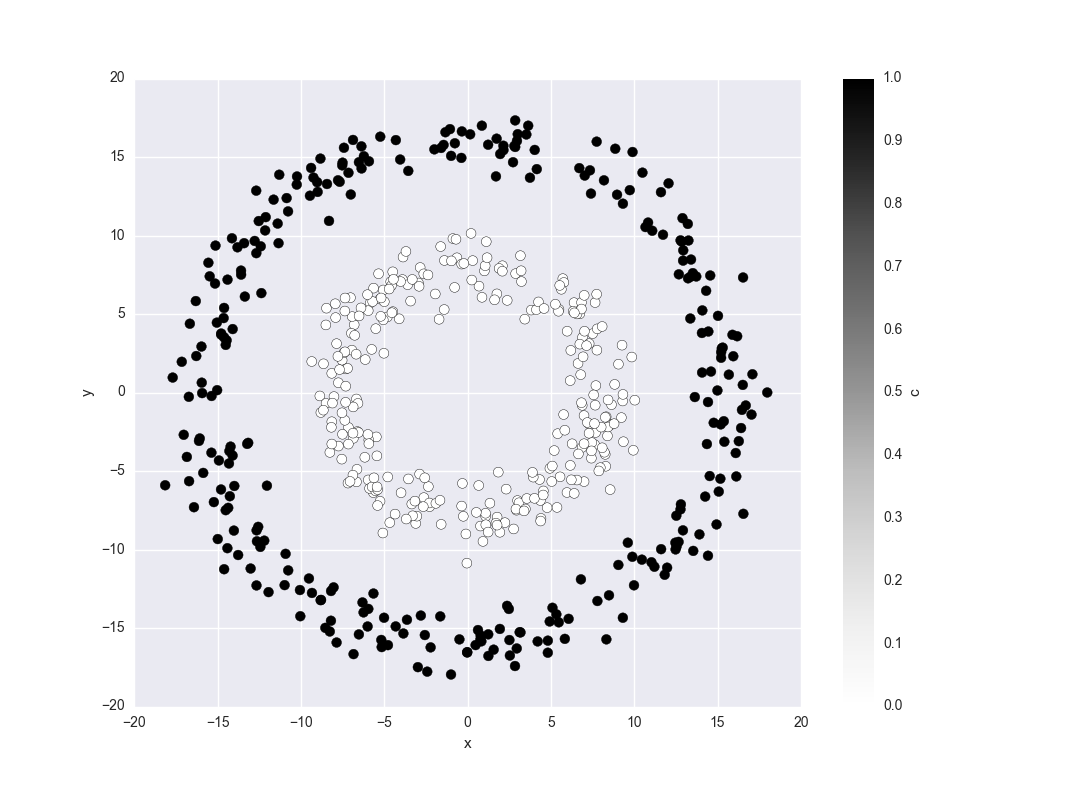
\includegraphics[scale=0.25]{circle_dataset.png} 
\end{center}
\end{frame}

\begin{frame}{Non linearity}
Not all patterns are linearly separable.
\begin{center}
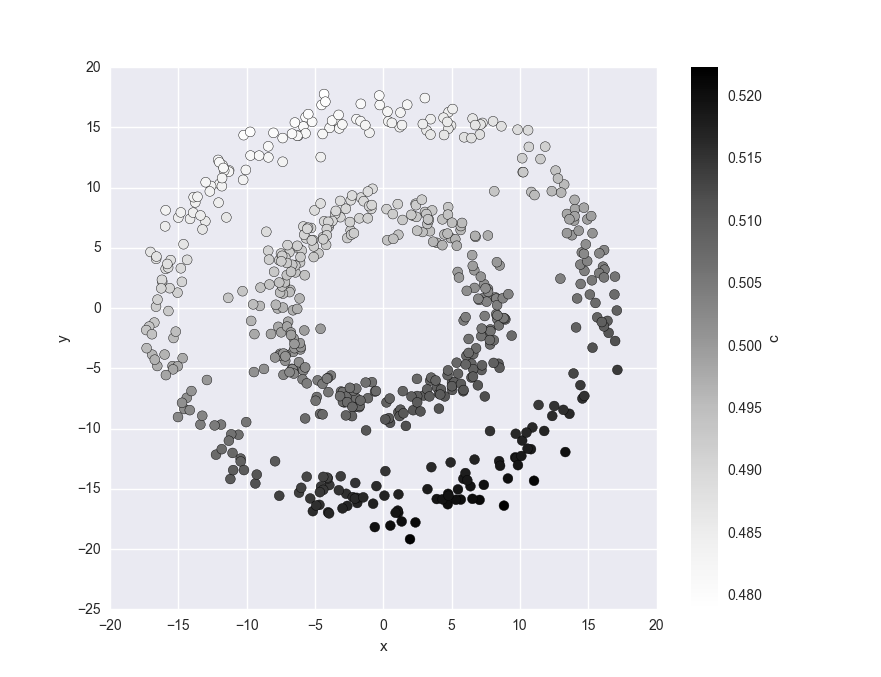
\includegraphics[scale=0.30]{circle_linear_model.png} 
\end{center}
\end{frame}

\begin{frame}{Kernels}
Theoretical justification for the use of kernels in linear models:
$$ L(X.\mu, y) \equiv L(XX^T.v, y) $$
Since $\mu$ is learned against $X$, $\mu$ can be spanned by $X$.

Most famous algorithm: kernel support vector classification.
\end{frame}


\begin{frame}{What a kernel machine sees (1/2) }
L2 Logistic regression, RBF kernel, nonlinear dataset:
\begin{columns}
\column{0.5\textwidth}
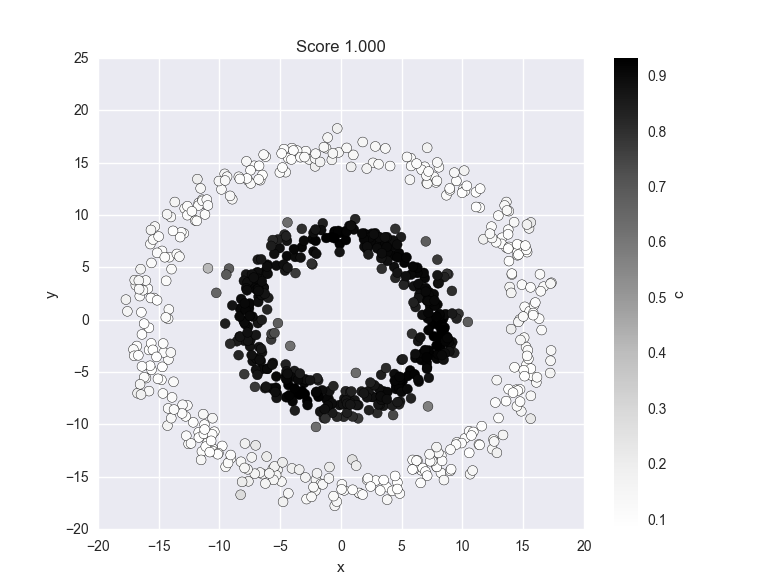
\includegraphics[scale=0.25]{circles_labels.png} 
\column{0.5\textwidth}
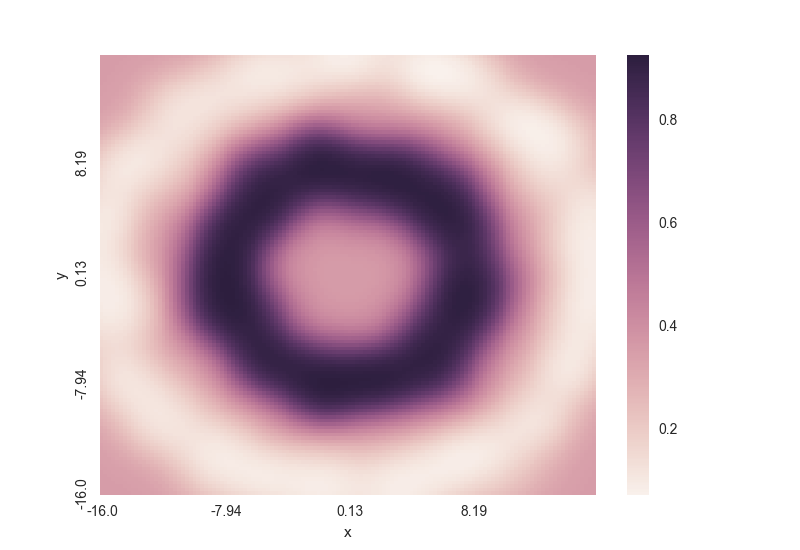
\includegraphics[scale=0.3]{circles_lenses.png} 
\end{columns}

\end{frame}

\begin{frame}{What a kernel machine sees (2/2) }
L2 Logistic regression, RBF kernel, arcs dataset:
\begin{columns}
\column{0.5\textwidth}
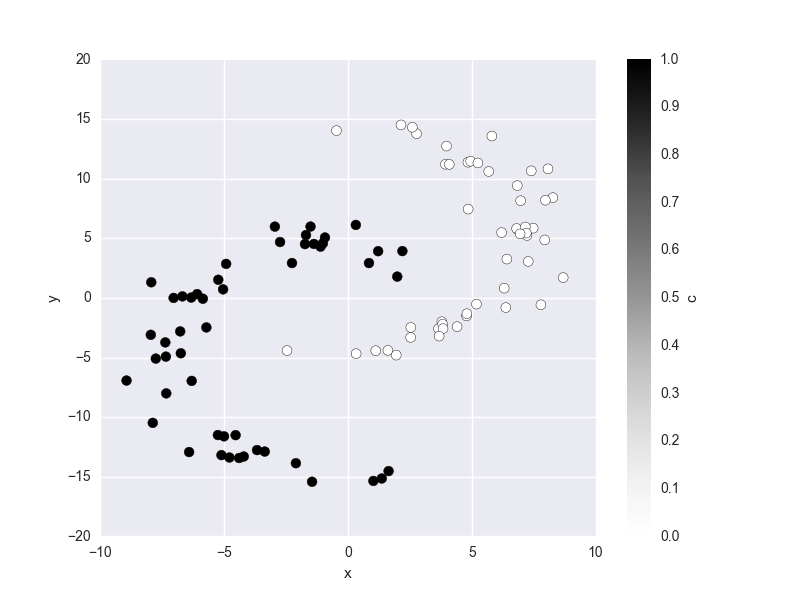
\includegraphics[scale=0.25]{arcs_labels.png} 
\column{0.5\textwidth}
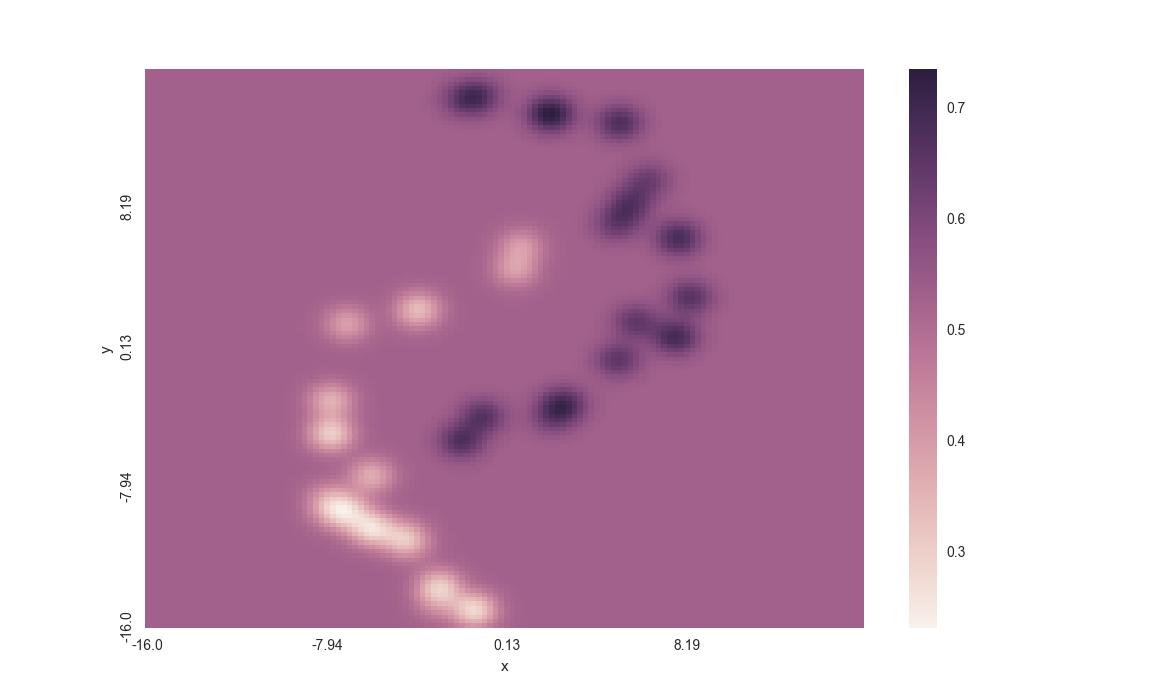
\includegraphics[scale=0.2]{arcs_lenses.png} 
\end{columns}
Here $\gamma$ (as in $K(x_1, x_2) = exp(-\gamma ||x1 - x2||^2)$) is chosen to highlight how the new feature space is built.
For each sample, the RBF kernel constructs a local indicator variable in the original feature space.
Each sample can become such a feature.
\end{frame}


\begin{frame}{Cogs in the kernel machine}
How a typical kernel decides how to classify a new sample $x_{new}$:
\begin{itemize}
\item $x_{new}$ is compared to the training $X = (x_1, x_2, \dots, x_n)$ using $K(., .)$.
\item The sample-to-sample distance $K(., .)$ makes use of the original feature space.
\item The kernel based features values $k = K(x_i, x_{new})$ are used for computing $y_{new} = v . k$. 
\end{itemize} 
\end{frame}

\begin{frame}{Weaknesses of kernels}
This leads to two points:
\begin{enumerate}
\item Often $K(., x)$ uses all the features in the original space, which as dimensionality grows, eventually scrambles relevant dimensions with the less relevant dimensions. 
\item Scalability issues (often $O(N^3)$ complexity)
\end{enumerate}
\end{frame}

\begin{frame}{Kernels with admixture of irrelevant features}
When all features (x, y) are relevant to the pattern:
\begin{columns}
\column{0.5\textwidth}
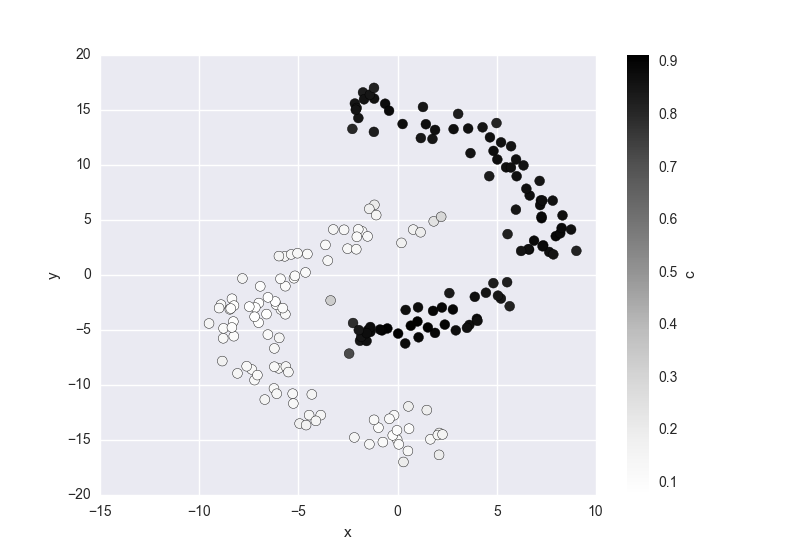
\includegraphics[scale=0.3]{kernel_dim_scale_0.png} 

\column{0.5\textwidth}
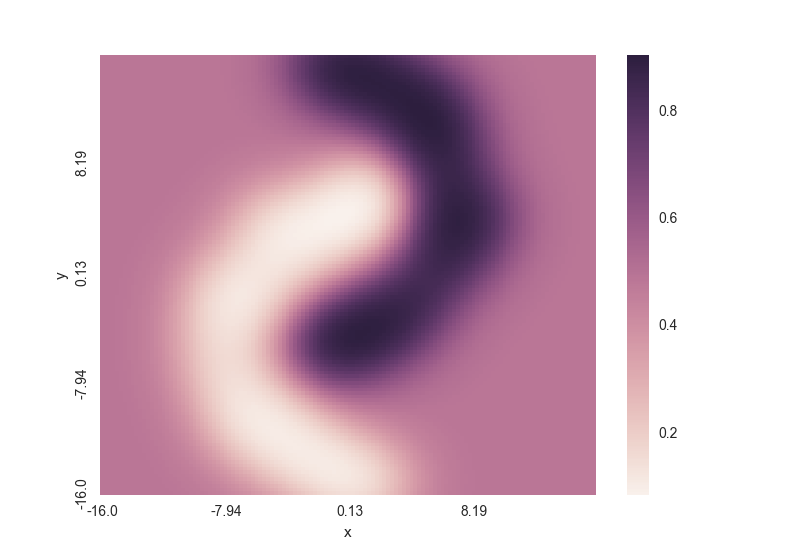
\includegraphics[scale=0.3]{kernel_dim_scale_0_hp.png} 

\end{columns}
\end{frame}

\begin{frame}{Kernels with admixture of irrelevant features}
When two irrelevant features are added (of similar variance):
\begin{columns}
\column{0.5\textwidth}
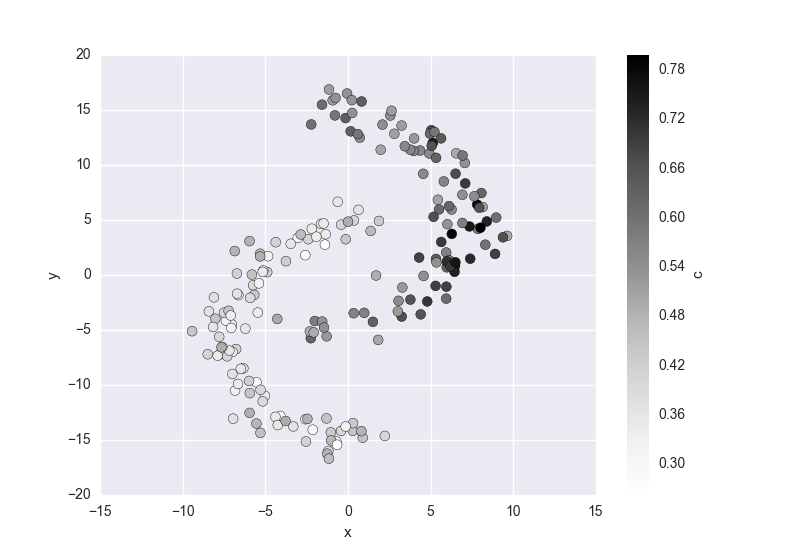
\includegraphics[scale=0.3]{kernel_dim_scale_2.png} 

\column{0.5\textwidth}
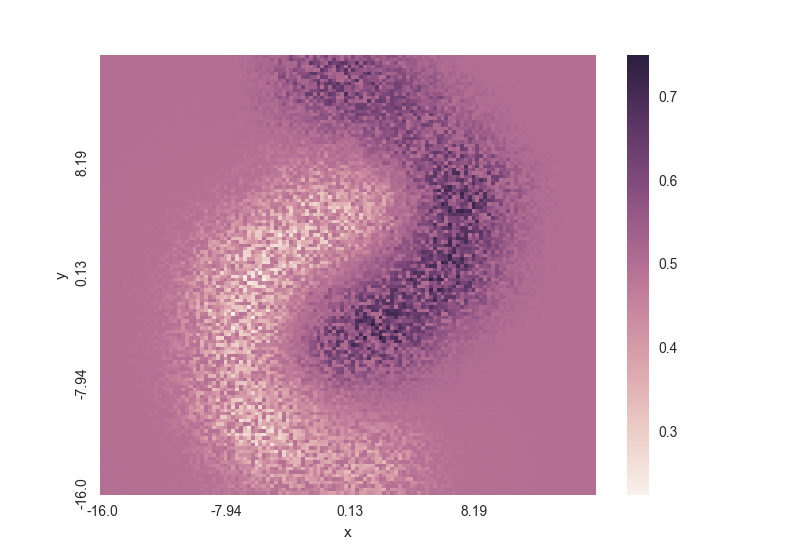
\includegraphics[scale=0.3]{kernel_dim_scale_2_hp.png} 

\end{columns}
\end{frame}

\begin{frame}{Kernels with admixture of irrelevant features}
When four irrelevant features are added (of similar variance):
\begin{columns}
\column{0.5\textwidth}
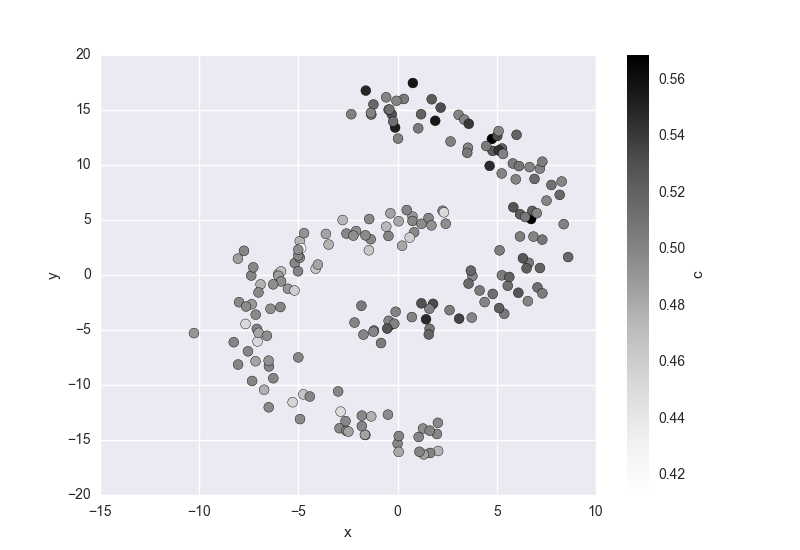
\includegraphics[scale=0.3]{kernel_dim_scale_4.png} 

\column{0.5\textwidth}
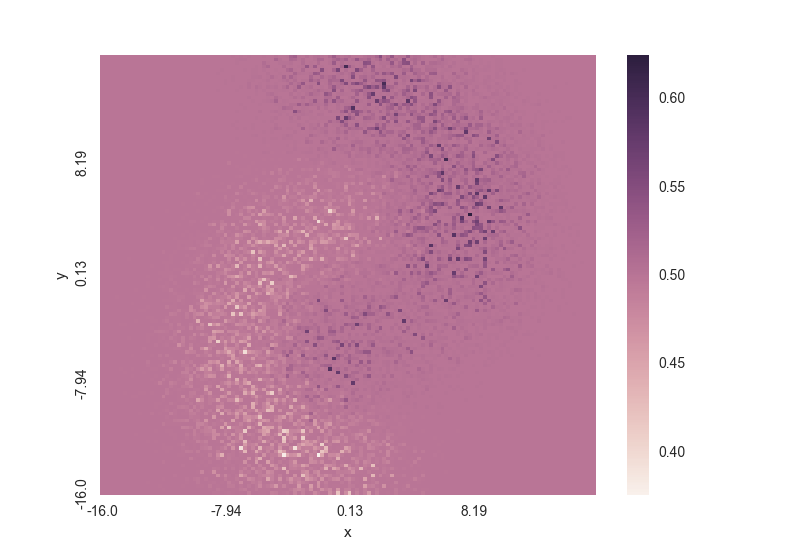
\includegraphics[scale=0.3]{kernel_dim_scale_4_hp.png} 
\end{columns}
The pure-kernel approach breaks down.
\end{frame}



\begin{frame}{Kernel machines weaknesses}
Mitigating kernel weaknesses (1):
\begin{enumerate}
\item High number of features: use only a subset of original features, where distances make sense.
\end{enumerate}
But how to bring in new information if we can't use new features?
\end{frame}

\begin{frame}{Explicit feature maps}
Explicit kernel transform step-by-step:
\begin{itemize}
\item Pick features from the original feature space which makes sense to include in kernel calculations.
\item Choosing "Interesting" samples, to promote as features $f_x(.) = K(., x)$ (lots of ways to be smart here!)
\item Augment (rather than replace) the original feature space with these features.
\end{itemize}
\end{frame}

\begin{frame}{Explicit feature maps}
L2 Logistic regression, "arcs" dataset, decision function for RBF kernel feature transform:
\begin{center}
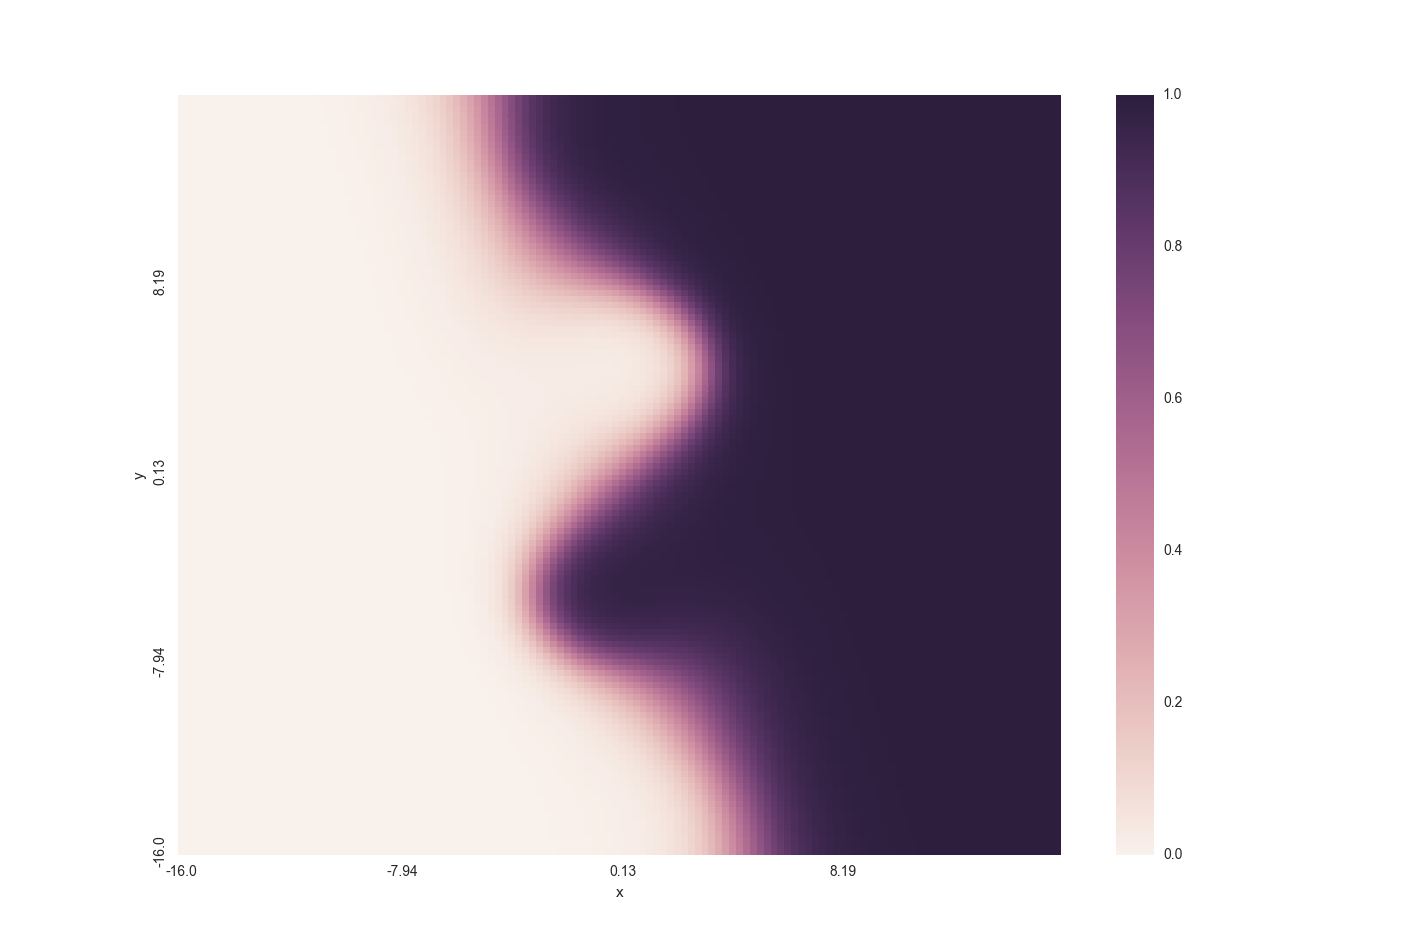
\includegraphics[scale=0.20]{arcs_transform.png}
\end{center}
\end{frame}

\begin{frame}{Explicit feature maps}
Decision function when the weights of the original features are erased after training (arcs dataset, RBF feature transform, L2 Logistic regression):
\begin{center}
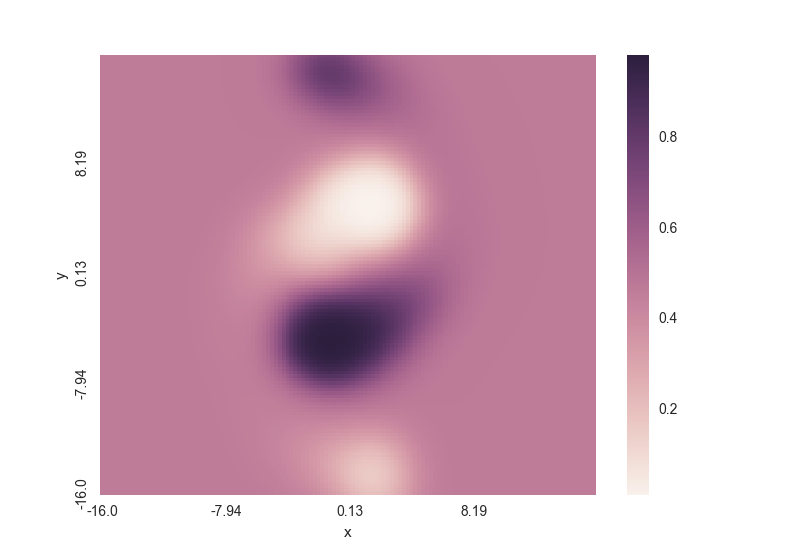
\includegraphics[scale=0.40]{arcs_sparsity.png}
\end{center}
Only some of the new kernel features are used, where linear features don't work.
\end{frame}

\begin{frame}{Kernels with admixture of irrelevant features}
Original features augmented with an explicit mapping of kernel features, four irrelevant features added:
\begin{columns}
\column{0.5\textwidth}
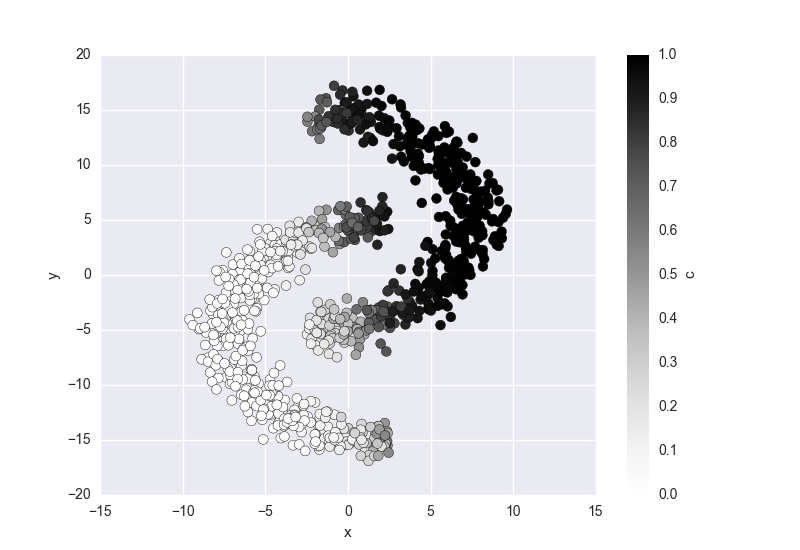
\includegraphics[scale=0.3]{kernel_dim_scale_4_lin.png} 

\column{0.5\textwidth}
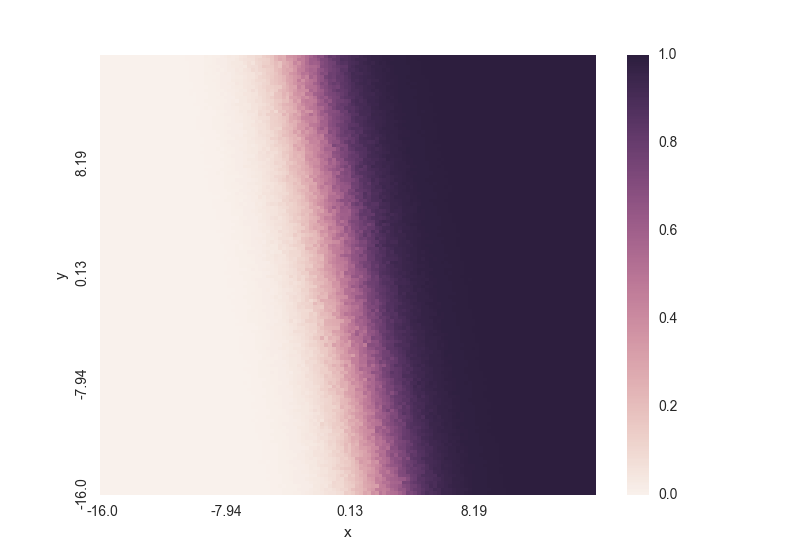
\includegraphics[scale=0.3]{kernel_dim_scale_4_hp_lin.png} 
\end{columns}
In this case, the kernel features break down too, but the model returns to a linear treatment.
\end{frame}

\begin{frame}{Kernel machines weaknesses}
Mitigating kernel weaknesses (2):
\begin{enumerate}
\item Scalability issues: use kernel approximation.
\end{enumerate}
\end{frame}

\begin{frame}{Addressing scalability issues}
Nystroem sampling:
\begin{itemize}
\item Approximates any kernel. 
\item Based on sampling \& interpolation.
\end{itemize}
 
\end{frame}

\begin{frame}{Addressing scalability issues}
For linear classification \& regression purposes, it is (mostly) equivalent to picking random samples as features as opposed to promoting all the samples.
\begin{figure}[h]
\begin{center}
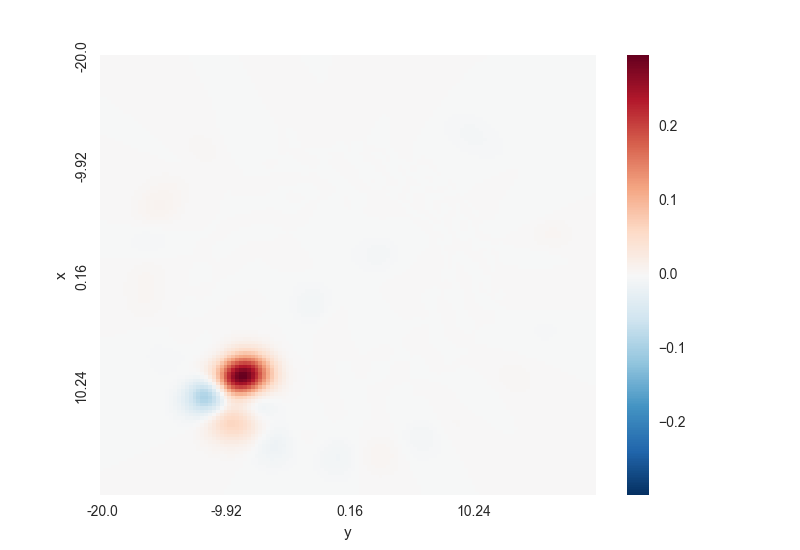
\includegraphics[scale=0.3]{nystroem_dimension.png}
\end{center}
\caption{A Nystroem dimension.}
\end{figure} 

\end{frame}


\begin{frame}{Addressing scalability issues}
Nystroem sampling in action, L2 Logistic regression, 50 kernel dimensions \& 100 samples:
\begin{columns}
\column{0.5\textwidth}
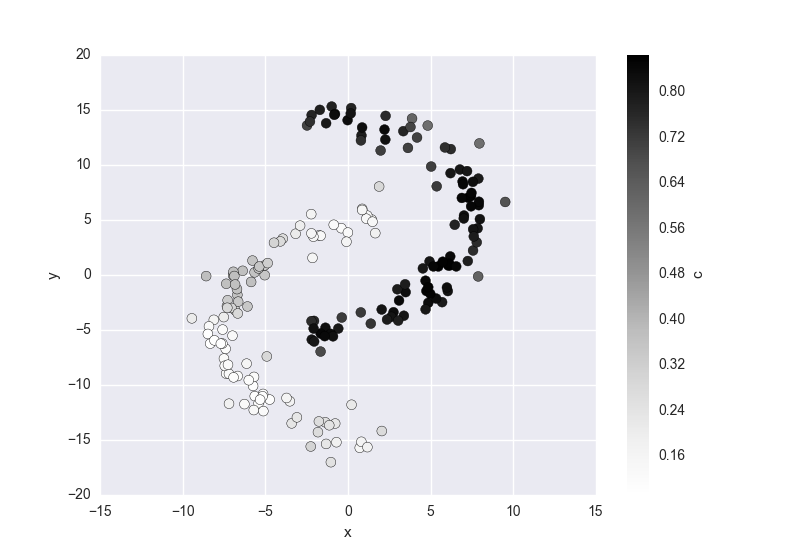
\includegraphics[scale=0.3]{arcs_nystroem.png} 

\column{0.5\textwidth}
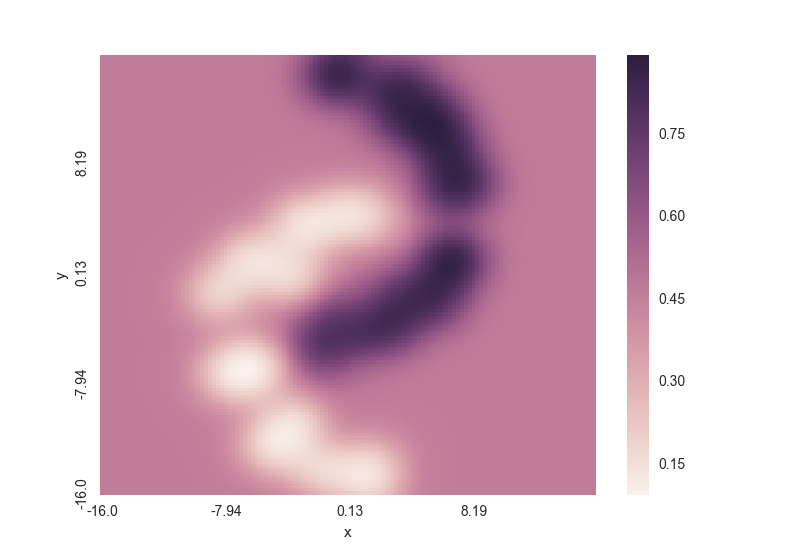
\includegraphics[scale=0.3]{arcs_nystroem_hm.png} 
\end{columns}
\end{frame}

\begin{frame}{Addressing scalability issues}
Nystroem sampling breaking down, L2 Logistic regression, 10 kernel dimensions \& 100 samples:
\begin{columns}
\column{0.5\textwidth}
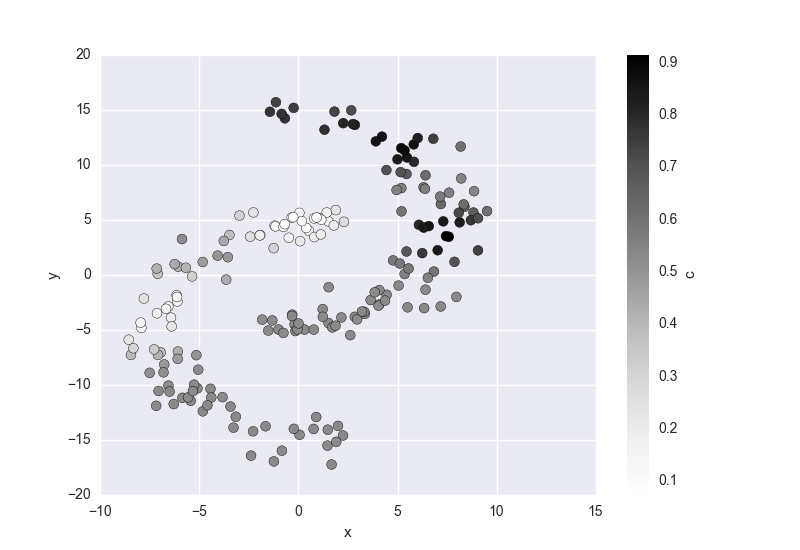
\includegraphics[scale=0.3]{arcs_nystroem_low.png} 

\column{0.5\textwidth}
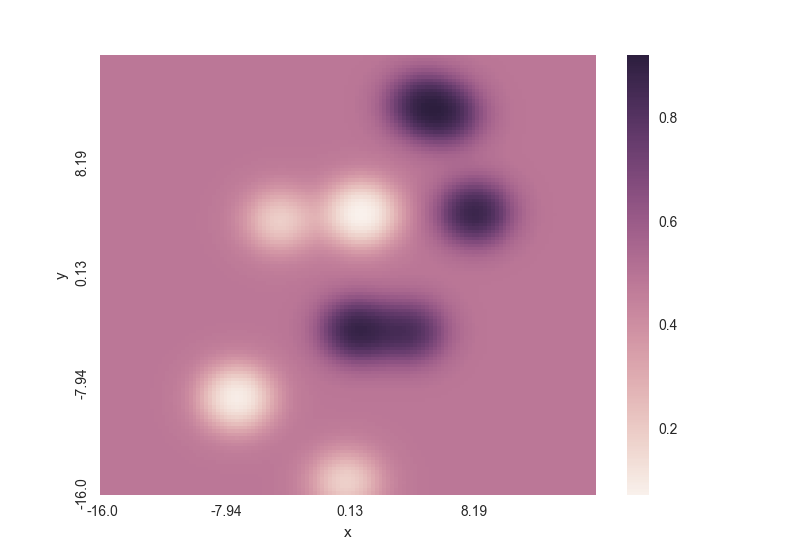
\includegraphics[scale=0.3]{arcs_nystroem_hm_low.png} 
\end{columns}
Important note: vanilla Nystroem sampling is unsupervised and does not attempt to find the best samples to pick.
\end{frame}


\begin{frame}{Addressing scalability issues}
Alternative, Fourrier RBF kernel approximation
\begin{columns}
\column{0.5\textwidth}
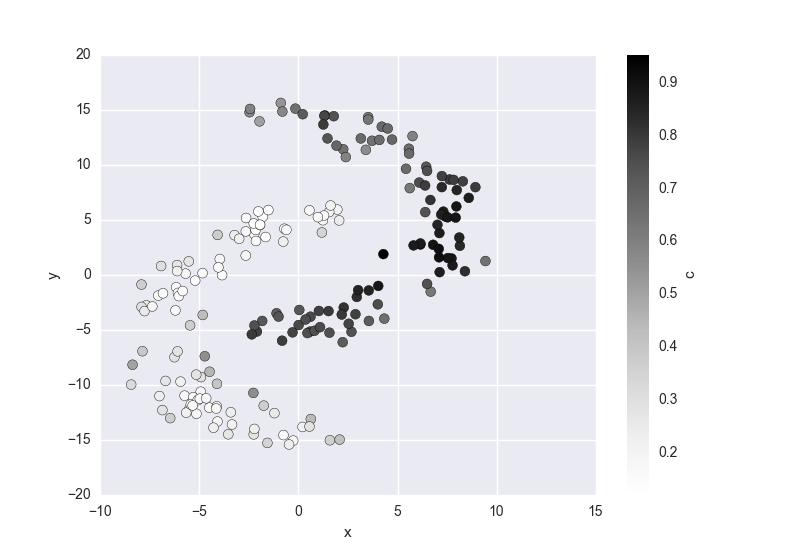
\includegraphics[scale=0.3]{arcs_rbfsampler.png} 

\column{0.5\textwidth}
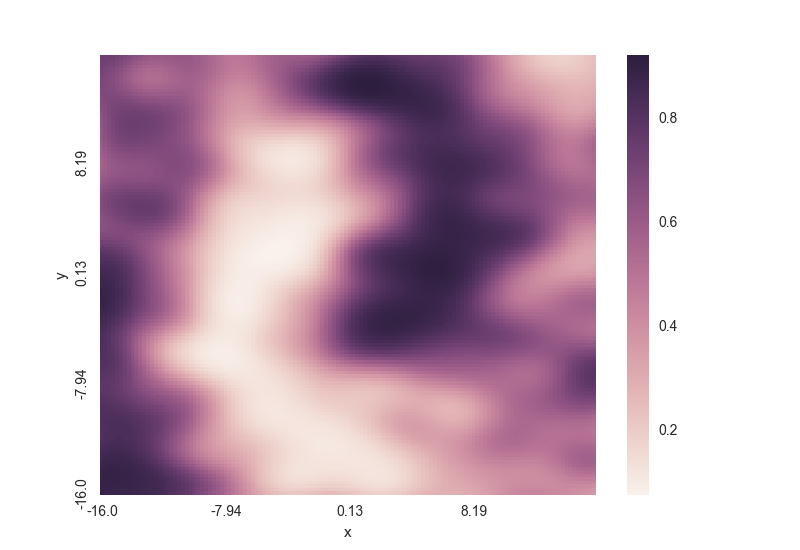
\includegraphics[scale=0.3]{arcs_rbfsampler_hm.png} 
\end{columns}

\end{frame}

\begin{frame}{Addressing scalability issues}
Fourrier RBF kernel approximation, zooming out:
\begin{center}
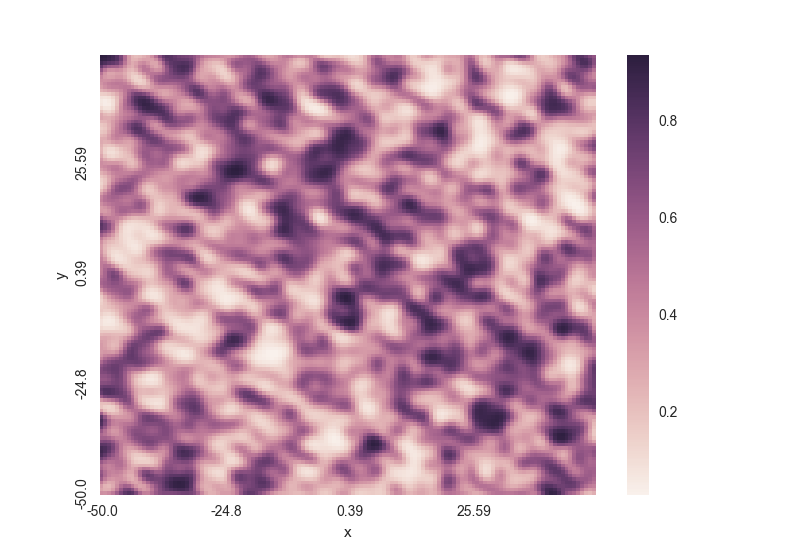
\includegraphics[scale=0.3]{arcs_rbfsampler_above.png} 
\end{center}
\end{frame}

\begin{frame}{Addressing scalability issues}
You can make your own kernel specific approximation, promote samples based on:
\begin{itemize}
\item Feature space coverage.
\item Where it helps the loss function.
\end{itemize}
Optionally go through a step of Nystroem or Cholesky for "normalization".

\end{frame}

\begin{frame}{Kernels wrap up}
Kernels allow non linear learning, and explicit mappings allows:
\begin{itemize}
\item Properly taking into account new features.
\item Gives a lot of engineering latitude in limiting the dimension of the new feature space by sampling.
\end{itemize}
\end{frame}

\begin{frame}{Non linearity II}
Special cases of non-linearity merit special treatment:
\begin{itemize}
\item per-feature internal structure.
\item particular features combinations.
\end{itemize}
\pause
Feature engineering helps with specialized feature transforms:
\begin{itemize}
\item Split a feature in binary bins (indicator variables) or linear steps (within-bin barycentric coordinates).
\item Bins extend to feature pairs (products of feature bin indicators).
\end{itemize}
\end{frame}

\begin{frame}{Non linearity II}
How to find these relevant combinations systematically, and optimally?
\pause
We need a supervised feature transform.
\end{frame}



\begin{frame}{Boosting feature transform}
Original features augmented with boosting features, L2 Logistic regression:
\begin{columns}
\column{0.5\textwidth}
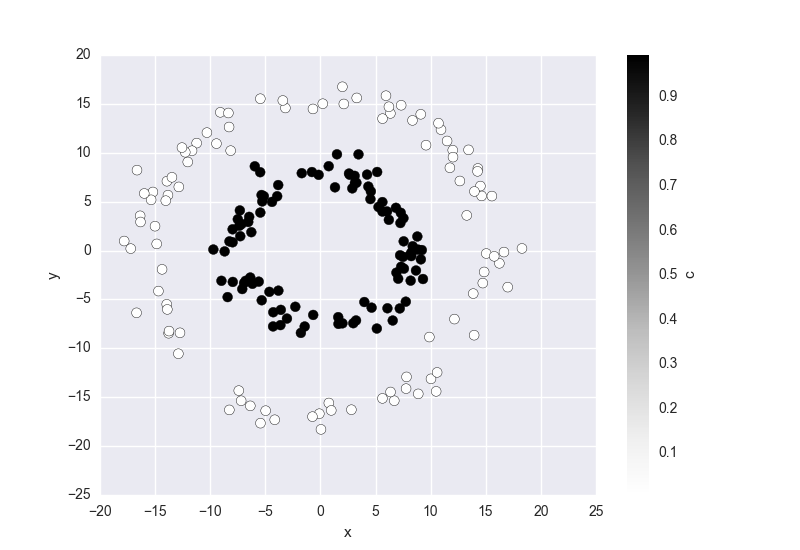
\includegraphics[scale=0.3]{circles_boosting.png} 

\column{0.5\textwidth}
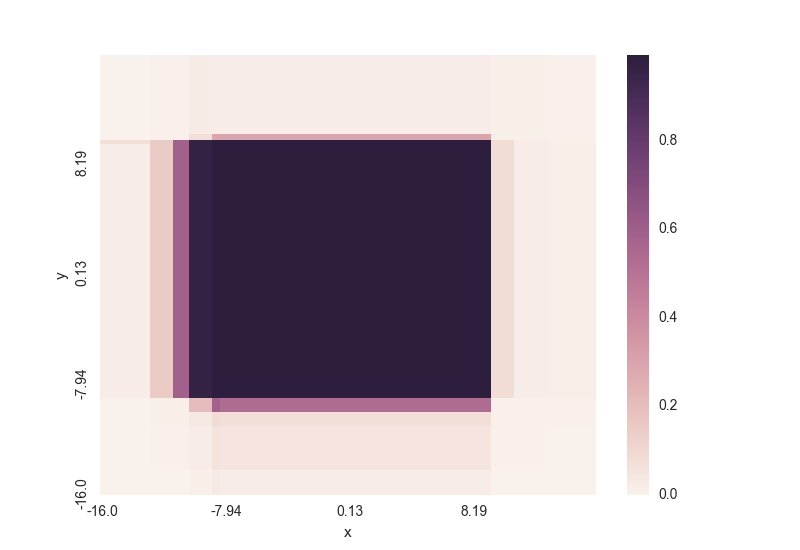
\includegraphics[scale=0.3]{circles_boosting_hm.png} 
\end{columns}
\end{frame}

\begin{frame}{Boosting feature transform}
Original features augmented with boosting features, L2 Logistic regression:
\begin{columns}
\column{0.5\textwidth}
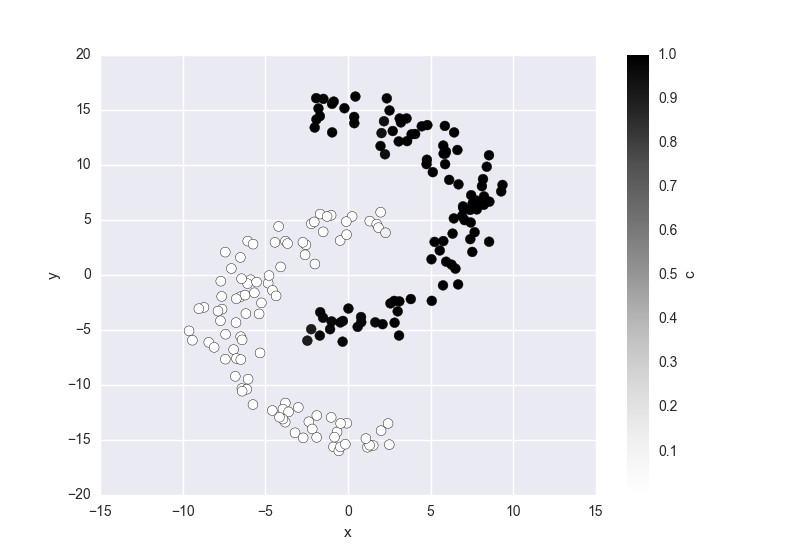
\includegraphics[scale=0.3]{arcs_boosting.png} 

\column{0.5\textwidth}
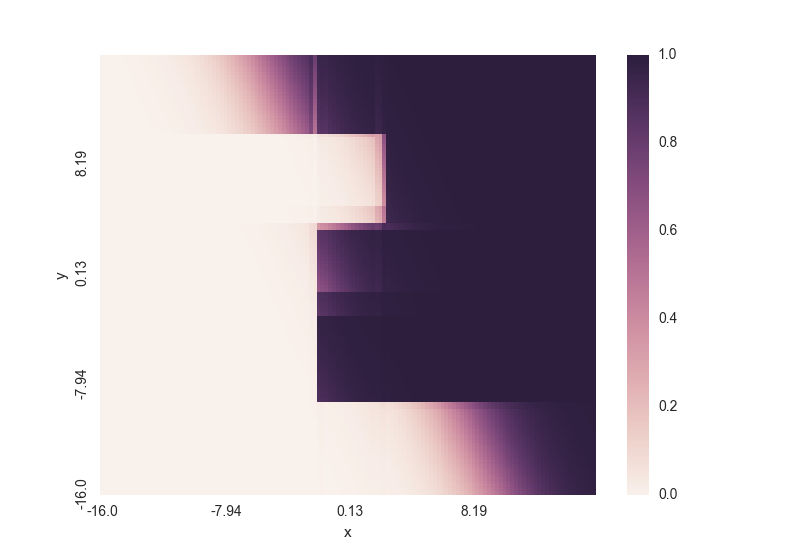
\includegraphics[scale=0.3]{arcs_boosting_hm.png} 
\end{columns}
\end{frame}

\begin{frame}{Boosting transforms basics}
What is a boosting transform:
\begin{itemize}
\item Train a gradient boosting model.
\item Each leaf of each tree is an indicator variable.
\item Augment the initial feature space with the leaf indicators as features.
\end{itemize}
They are the workhorse of CTR prediction at Facebook (see ADKDD 2014)
\end{frame}

\begin{frame}
Boosting feature transform analogies:
\begin{itemize}
\item one-level tree (decision stump): analogous to feature bin indicator.
\item multiple branching levels: analogous to feature tuples.
\item minimum samples per leaf: analogous to quantile binning.
\end{itemize}
\end{frame}

\begin{frame}{Boosting transforms pros \& cons}
Boosting transform are great, they are 
\begin{itemize}
\item Sparse.
\item Supervised: mostly no need to worry about irrelevant features.
\item A bit rough around the edges...
\end{itemize}
\end{frame}

\begin{frame}{Boosting \& Mixed classes}
L2 Logistic regression, boosting transform alone vs boosting plus RBF features
\begin{columns}
\column{0.5\textwidth}
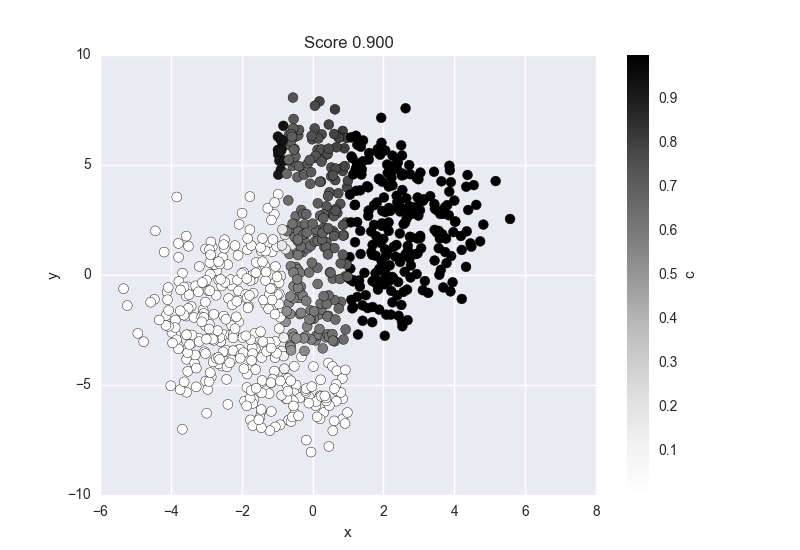
\includegraphics[scale=0.3]{boosting_only.png} 

\column{0.5\textwidth}
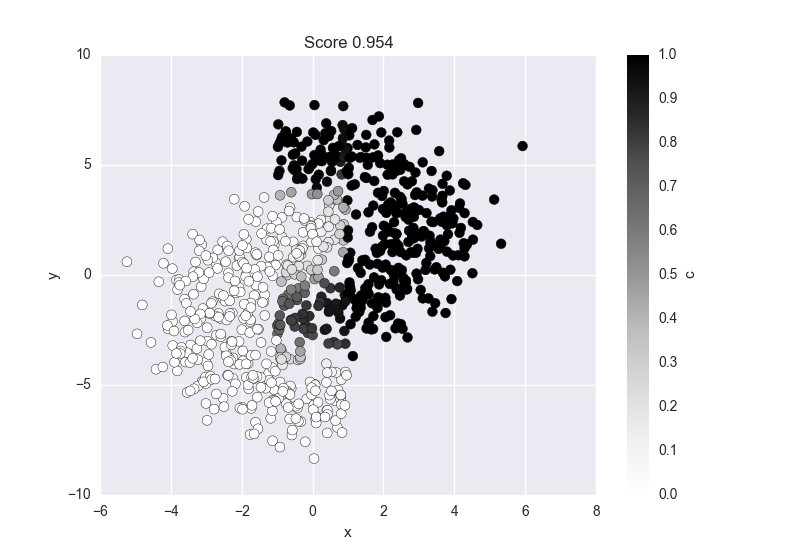
\includegraphics[scale=0.3]{boosting_nys_labels.png} 
\end{columns}

\end{frame}

\begin{frame}{Boosting \& Mixed classes}
L2 Logistic regression, boosting transform alone vs boosting plus RBF features
\begin{columns}
\column{0.5\textwidth}
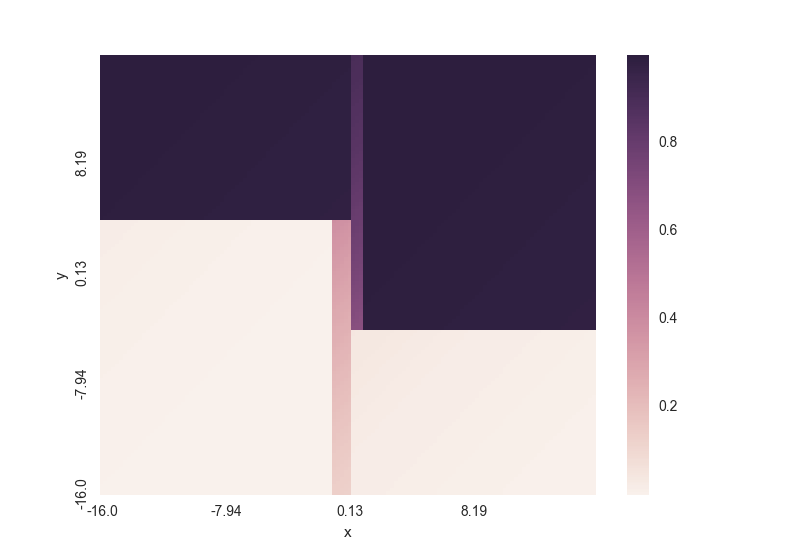
\includegraphics[scale=0.3]{boosting_only_hm.png} 

\column{0.5\textwidth}
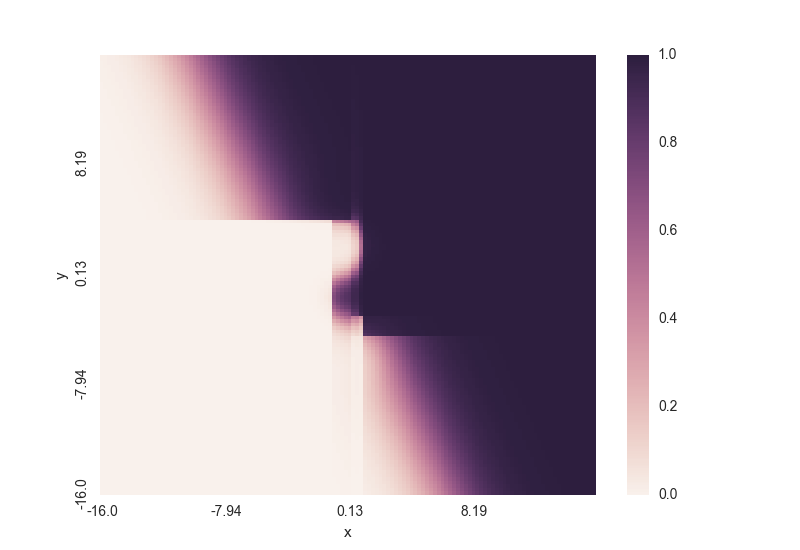
\includegraphics[scale=0.3]{boosting_nys_hm.png} 
\end{columns}

\end{frame}

\begin{frame}{Conclusion}
An approach based on composable feature transforms, with:
\begin{itemize}
\item Linear learning core (with all the benefits)
\item Feature transforms create a white box, supervised map of the feature space.
\item Feature transforms operate correctly side by side, with other transforms and with linear features.
\end{itemize}
It contrasts with the "pick the right black box" approach.

Code on github \url{https://github.com/borithefirst/epfl_pres/blob/master/code/kernel_lin.py}
\end{frame}

\end{document}